\documentclass{standalone}
\usepackage{tikz}
\usepackage{ctex,siunitx}
\usepackage{tkz-euclide}
\usepackage{amsmath}
\usetikzlibrary{patterns, calc}
\usetikzlibrary {decorations.pathmorphing, decorations.pathreplacing, decorations.shapes,}
\begin{document}
\small
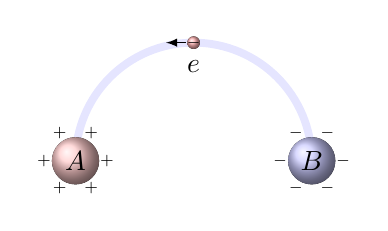
\begin{tikzpicture}[>=latex,scale=1.0]
  \draw[line width=1mm,blue!10](-1.5,0)arc(180:0:1.5);
  \fill[ball color=red!20](-1.5,0)circle(0.3)node{$A$};
  \fill[ball color=blue!20](1.5,0)circle(0.3)node{$B$};
  \fill[ball color=red!30](0,1.5)circle(0.08)node{\tiny$-$};
  \foreach \x in {0,60,...,300}
  {
    \node at ([shift=(\x:0.4cm)]-1.5,0){\tiny$+$};
    \node at ([shift=(\x:0.4cm)]1.5,0){\tiny$-$};
  }
  \draw[->](-0.1,1.5)--++(-0.25,0);
  \node at (0,1.5)[below=1mm]{$e$};
\end{tikzpicture}
\end{document}